
%(BEGIN_QUESTION)
% Copyright 2012, Tony R. Kuphaldt, released under the Creative Commons Attribution License (v 1.0)
% This means you may do almost anything with this work of mine, so long as you give me proper credit

Danger Dave decides to outfit his car with a solid-fuel rocket mounted in the trunk.  Unfortunately, he can't get the rocket motor to fit horizontally in the trunk, and so it sits at a slight angle (15 degrees from horizontal).  When the rocket is ignited, its thrust is 3400 pounds of force along the centerline of the rocket body:

$$\includegraphics[width=15.5cm]{i02615x01.eps}$$

One fine day, Dave is feeling particularly dangerous, so he ignites the rocket motor to see how fast his car will perform on a quarter-mile racetrack.  Calculate the amount of work done by the rocket on the car during the quarter-mile run.

\vskip 10pt

Assuming Dave's car weighs 3100 pounds (i.e. it has a {\it mass} of 96.27 slugs) with the new rocket motor installed and him in the driver's seat, calculate both his quarter-mile speed and time.  Hint: you may need to use one or more of these formulae:

$$F = ma$$

$$x = vt$$

$$v = at + v_0$$

$$x = {1 \over 2} at^2$$

\noindent
Where,

$F$ = Force applied to object

$m$ = Mass of object

$x$ = Position of object with reference to a starting point ($x_0$, at time $t$ = 0)

$v$ = Velocity of object

$a$ = Acceleration of object (i.e. the rate at which velocity changes)

$t$ = Elapsed time

$v_0$ = Initial velocity of object (at time $t$ = 0)

\vskip 10pt

\underbar{file i02615}
%(END_QUESTION)





%(BEGIN_ANSWER)

The work done by the rocket motor on the car may be calculated with the work formula, taking the displacement ($x$) to be one-quarter of a mile (1320 feet):

$$W = F x \cos \theta$$

$$W = (3400 \hbox{ lb}) (1320 \hbox{ ft}) \cos 15^o$$

$$W = \hbox{4335075.1 ft-lb of work done on Dave's car}$$

\vskip 10pt

The horizontal component of the rocket's 3400 lb thrust will be the 3400 lb times the cosine of 15 degrees:

$$F_x = (3400 \hbox{ lb}) \cos 15^o = 3284.15 \hbox{ lb}$$

The acceleration of Dave's car with this amount of force driving it down the racetrack will be equal to force divided by mass, following the formula $F = ma$.  In order to calculate $a$, we will need to know the mass of Dave's car in slugs (3100 lb / 32.3 ft/s$^{2}$ = 96.27 slugs):

$$F = m a$$

$$a = {F \over m} = \left(3284.15 \hbox{ lb} \over 96.27 \hbox{ slugs}\right) = 34.11 \hbox{ ft/s}^2$$

To put this in perspective, the car would accelerate at 32.2 ft/s$^{2}$ {\it if pushed off a cliff}, so this means Dave's car will ``rocket'' down the racetrack at an acceleration faster than free-fall!

\vskip 10pt

The distance traveled ($x$) by an object under constant acceleration ($a$) is given by the following formula:

$$x = {1 \over 2} a t^2$$

In the case of Dave's rocket car:

$$1320 \hbox{ ft} = {1 \over 2} (34.11 \hbox{ ft/s}^2) t^2$$

Solving for time ($t$):

$$t^2 = {(2) (1320 \hbox{ ft}) \over (34.11 \hbox{ ft/s}^2)}$$

$$t = \sqrt{(2) (1320 \hbox{ ft}) \over (34.11 \hbox{ ft/s}^2)}$$

$$t = 8.797 \hbox{ seconds}$$

This, my friends, is a very respectable quarter-mile time!

\vskip 10pt

\filbreak

As for top speed (at the end of the quarter-mile run, since we assume Dave is still accelerating with the rocket motor going at full thrust), this may be calculated by the velocity-acceleration formula $v = at$:

$$v = at$$

$$v = (34.11 \hbox{ ft/s})(8.797 \hbox{ s}) = 300.1 \hbox{ ft/s}$$

This happens to be 204.6 miles per hour, which again is {\it very respectable} in a quarter-mile race!

\vskip 10pt

Now, Dave's only real problem is how to stop.

%(END_ANSWER)





%(BEGIN_NOTES)


%INDEX% Physics, energy, work, power

%(END_NOTES)


